\chapter{Method}
\label{ch:architecture}
\section{Overview}
The framework of the study consists of four main stages: data collection, data preprocessing, data analysis, and modeling. Each stage is crucial to the analysis and modeling. Initially, data was collected from various open-source datasets. As such sources may contain potential inconsistencies, data preprocessing steps were employed to enhance the cleanliness of the gathered data. After the preprocessing phase, data analysis was conducted to understand the dataset's characteristics better. This includes identifying keyword occurrences and conducting sentiment analysis. Following data analysis, various deep learning models were trained and evaluated. The performance of these models was compared against traditional text classification methods and state-of-the-art LLM models to estimate the effectiveness and performance of different methods within the context. An innovative fusion of ensemble learning techniques was employed to improve detection performance further by using a fuzzy rank-based ensemble approach with the Gompertz function. This approach used a fuzzy rank-based ensemble approach with the Gompertz function. The technique allowed for the adjustment of weights based on the confidence scores of each classifier. The result was more robust and reliable predictions for each sample, which enhanced the overall accuracy of the prediction processes used in the study.

\section{Data Collection}
All text data used in this study were collected from open-source datasets, famous fact-checking websites, and reliable official websites. The gathered data were filtered by using keywords associated with long COVID and reinfection, such as chronic, long-term, persistent, after-effects, sequelae, complications, recovery, post covid, post-covid, omicron, subvariant, reinfection, immune, and variant. The resulting collection formed the dataset for the following experiments. Each sample of data was categorized as either "genuine" or "fake".

\subsection{Open-source datasets}
\textbf{Fighting an Infodemic\cite{b4}:}
An earlier dataset contains topics related to COVID-19 sourced from platforms like Facebook, Twitter,  and websites for fact-checking. This dataset was selected for the \textit{Constraint@AAAI2021 - COVID19 Fake News Detection in English competition}. Only labeled samples from the dataset were used, available on GitHub repository\cite{b9}.\\

\textbf{COVID-19 Twitter Fake News (CTF)\cite{b6}:}
CTF is a dataset focused on tweets from the social media platform Twitter. It includes both labeled and unlabeled data about genuine and fake COVID-19 news. In addition, this dataset contains the tweeters' user-profile features. For this study, only data with label and text content was used.\\

\textbf{Covid-19 heAlthcare mIsinformation Dataset (CoAID)\cite{b10}}:
The CoAID dataset is a collection of COVID-19 fake news sourced from the internet and social media platforms such as Twitter. It includes news articles, user engagements related to fake messages, tweets, and labels.\\


\textbf{Fake news information-broadcasting dataset of COVID-19 (FibVID )\cite{b11}}:
The dataset collects claims from fact-checking websites such as Snopes and Politifact and some related discussions from Twitter. It also assembles user profile data from social media platforms. The FibVID includes COVID and non-COVID topics, separated into four labels. Only samples related to COVID-19 from categories 0 and 1 were used.\\

\textbf{FaCOV\cite{b12}}:
This dataset gathered from 13 English fact-checking websites related to COVID-19, includes article titles, claims made within the articles, external links, and abstracts. The titles and contents from articles were merged, and data with two category labels were used in the experiments.

\subsection{Fact-checking websites}
While open-source databases provide significant help, most contain data only from 2019 to 2021. To conquer this limitation, web scraping and data cleaning techniques were used to gather more recent data. The data collection process comprised the following steps: choosing reliable data sources, extracting text data from websites, and labeling the collected data.\\

\textbf{Source:}
Snopes\cite{b13} and PolitiFact\cite{b14}, both verified by the International Fact-Checking Network (IFCN), were chosen as our primary data sources. This certification assures the audience that the data and labels from these sites have undergone transparent and strict validation processes, enhancing reliability.\\

\textbf{Extraction:}
Given the vast amount of target data, a systematic approach was employed using web scraping to extract articles tagged as  'CORONAVIRUS' and 'COVID-19' from PolitiFact (data up to July 31, 2023) and Snopes (data up to August 31, 2023). The approach was to collect the article contents and the labels for model training. Considering that many articles on fact-checking websites are false news, the clarifications were collected as True samples to balance the ratio if an article was classified as False. From Snopes and PolitiFact, we extracted 1500 and 806 texts, respectively. Later, the collected data were filtered by keywords to align more closely with the research topic. Fig. \ref{fig:fack-checking websites} shows the example of collecting data from PolitiFact.\\

\textbf{Labeling:}
Snopes classifies articles into fourteen labels: lost-legend, labeled-satire, legend, scam, misattributed, correct-attribution, miscaptioned, outdated, unproven, false, mostly false, mixture, mostly-true, and true. On the other hand, PolitiFact categorizes articles into six labels: true, mostly-true, half-true, barely-true, false, and pants-on-fire. According to the study by Khan et al.\cite{b15}, the labels from different databases were reclassified into two categories: genuine and fake. Specifically, the claims labeled as labeled-satire, scam, miscaptioned, misattributed, mostly-false, barely-true, false, and pants-on-fire were categorized as fake. In contrast, those with other labels were categorized as true. Claims with unproven or mixture labels from Snopes were not involved\cite{b11}. 

\begin{figure}
  \centering
  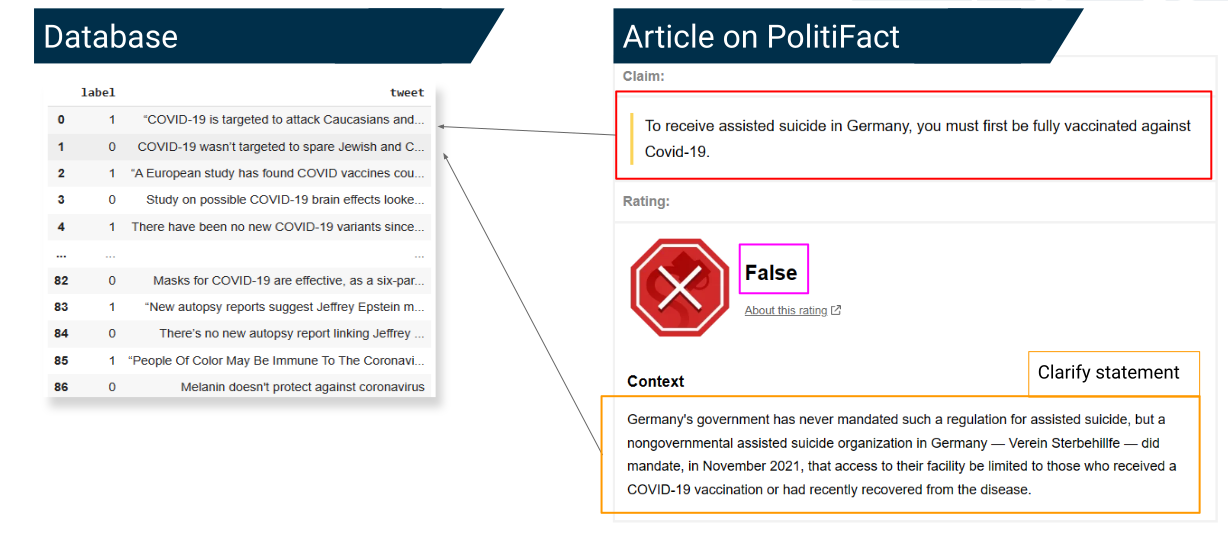
\includegraphics[width=1\columnwidth]{img/fack-checking websites.png}
  \caption{The example of collecting data from fact-checking websites(PolifiFact). } 
  \vspace{-0.4cm}
  \label{fig:fack-checking websites}
\end{figure}

\subsection{Governmental bodies}
Highly reputable government and public organization websites, such as the Centers for Disease Control and Prevention (CDC) and the World Health Organization (WHO), were also considered primary sources. These organizations have consistently supplied up-to-date information and guidelines during the pandemic, so they are widely considered authentic and reliable data sources. 
The articles related to "long COVID" and "Reinfection" were gathered from the COVID-19 sections of these websites. Considering that the original text might have needed longer or included unnecessary details, we utilized ChatGPT \cite{b8} to refine the acquired content. Using ChatGPT, we organized and structured the texts to ensure each claim had an appropriate length and clarity. As a result, each claim was labeled as "genuine" according to its reputable source. After these steps, the dataset used for model training included the latest information.
The table below presents the filtered sample counts from various data sources in Table \ref{tab:data_source}.

\begin{table}[]
    \caption{Sample size from different sources}
    \label{tab:data_source}
    \centering
\begin{tabular}{
>{\columncolor[HTML]{FFFFFF}}c 
>{\columncolor[HTML]{FFFFFF}}c 
>{\columncolor[HTML]{FFFFFF}}c 
>{\columncolor[HTML]{FFFFFF}}c 
>{\columncolor[HTML]{FFFFFF}}c }
\hline
{\color[HTML]{000000} \textbf{Source}} & {\color[HTML]{000000} \textbf{Time until}} & {\color[HTML]{000000} \textbf{Samples}} & {\color[HTML]{000000} \textbf{Fake}} & {\color[HTML]{000000} \textbf{Genuine}} \\ \hline
{\color[HTML]{000000} CTF}             & {\color[HTML]{000000} $\sim$2021}          & {\color[HTML]{000000} 1292}             & {\color[HTML]{000000} 1130}          & {\color[HTML]{000000} 162}              \\
{\color[HTML]{000000} Fighting an Infodemic}            & {\color[HTML]{000000} $\sim$2021}          & {\color[HTML]{000000} 218}              & {\color[HTML]{000000} 62}            & {\color[HTML]{000000} 156}              \\
{\color[HTML]{000000} CoAID}           & {\color[HTML]{000000} $\sim$2020}          & {\color[HTML]{000000} 70}               & {\color[HTML]{000000} 0}             & {\color[HTML]{000000} 70}               \\
{\color[HTML]{000000} FibVID}          & {\color[HTML]{000000} $\sim$2020}          & {\color[HTML]{000000} 615}              & {\color[HTML]{000000} 318}           & {\color[HTML]{000000} 297}              \\
{\color[HTML]{000000} FaCOV}           & {\color[HTML]{000000} $\sim$2021}          & {\color[HTML]{000000} 811}              & {\color[HTML]{000000} 811}           & {\color[HTML]{000000} 0}                \\
{\color[HTML]{000000} PolitiFact}      & {\color[HTML]{000000} $\sim$2023}          & {\color[HTML]{000000} 87}               & {\color[HTML]{000000} 42}            & {\color[HTML]{000000} 45}               \\
{\color[HTML]{000000} Snopes}          & {\color[HTML]{000000} $\sim$2023}          & {\color[HTML]{000000} 15}               & {\color[HTML]{000000} 9}             & {\color[HTML]{000000} 6}                \\
{\color[HTML]{000000} CDC+WHO}         & {\color[HTML]{000000} $\sim$2023}          & {\color[HTML]{000000} 58}               & {\color[HTML]{000000} 0}             & {\color[HTML]{000000} 58}               \\ \hline
{\color[HTML]{000000} Total}           & {\color[HTML]{000000} }                    & {\color[HTML]{000000} 3166}             & {\color[HTML]{000000} 2372}          & {\color[HTML]{000000} 794}              \\ \hline
\end{tabular}
\end{table}

\section{Data Preprocessing}
This study executed three data preprocessing steps to ensure the integrity of the gathered dataset. Firstly, duplicate entries were removed by cross-referencing the merged open-source datasets with existing ones. This step eliminated redundancy, reinforcing confidence in data quality and preventing potential influences on subsequent model training and analysis. Secondly, emojis and external links (URLs), commonly found in social media posts, were cleaned to enhance clarity. Thirdly, label encoding was performed, with '0' representing genuine news and '1' representing fake news. Stratified sampling was employed, assigning 10\% of the data for testing and 90\% for training. This approach ensured consistent label proportions in both sets, reducing the potential shortage of genuine samples that might arise from random sampling.

\subsection{Remove duplicate entries}
To ensure the absence of duplicate entries in the merged open-source datasets, we cross-referenced the data with existing open-source datasets. Any identified duplicate samples were eliminated to reduce redundancy, reinforcing confidence in the data quality and preventing potential influences on the following model training and analysis performance.
\subsection{Remove emojis and URLs}
During the preprocessing phase, social media posts and articles, which frequently include emojis and external links (URLs), were processed to enhance the clarity of the dataset in distinguishing between genuine and fake news. The Tweet-preprocessor package\cite{b5} was employed to remove emojis and URLs from the texts (Fig. \ref{fig:preprocessing}).

\begin{figure}
  \centering
  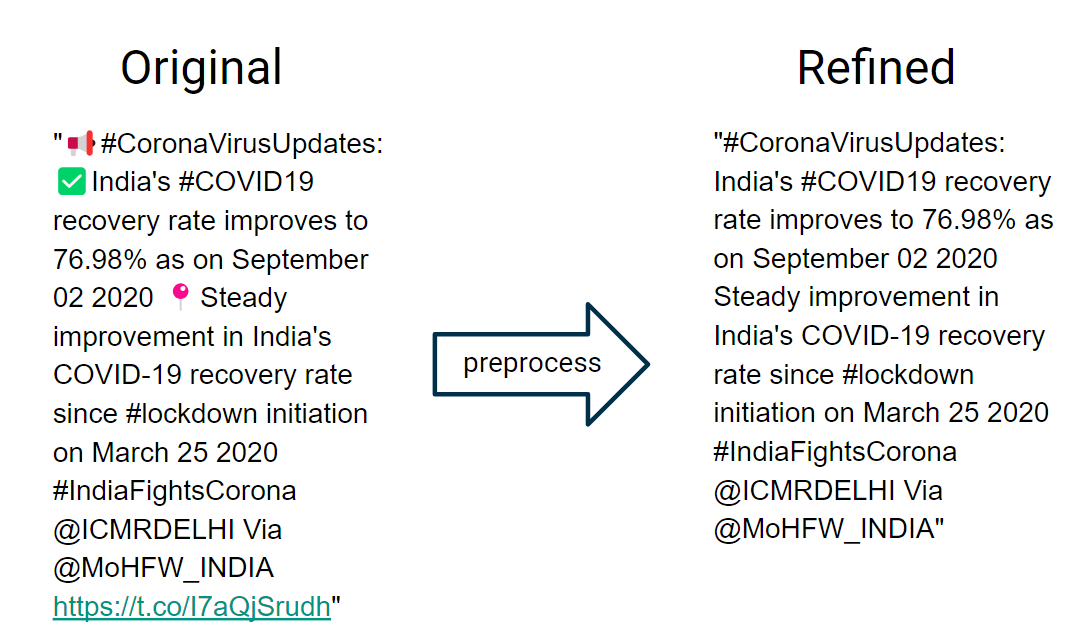
\includegraphics[width=1\columnwidth]{img/preprocessing.png}
  \caption{The example for removing emojis and URLs.} 
  \vspace{-0.4cm}
  \label{fig:preprocessing}
\end{figure}

\subsection{Label encoding}
All the labels were encoded as '0' (stands for genuine) and '1' (stands for fake), respectively. The distribution of our dataset is illustrated in Fig. \ref{fig:data distribution}. As the public data sources exhibited a bias towards the 'fake' category, an imbalanced label distribution was observed in the dataset. To ensure fairness, we employed stratified sampling, allocating 10\% of the data for testing and 90\% for training. This sampling approach ensures consistent label proportions in both the test and training sets, preventing the potential insufficient of genuine samples that may arise from random sampling.



\begin{figure}
  \centering
  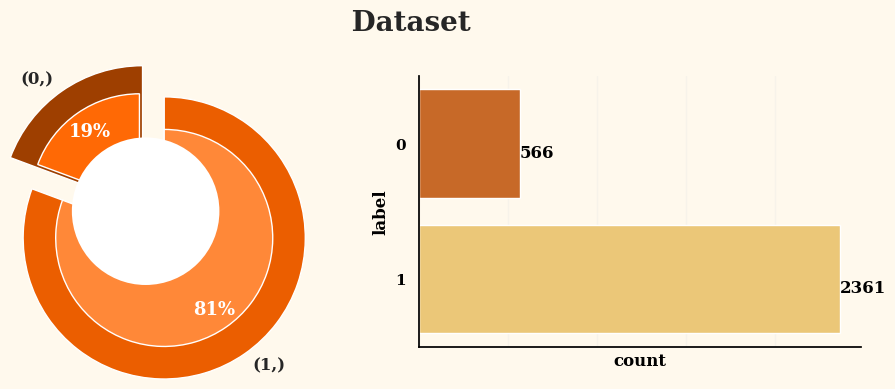
\includegraphics[width=1\columnwidth]{img/data distribution.png}
  \caption{Label distribution after preprocessing.} 
  \vspace{-0.4cm}
  \label{fig:data distribution}
\end{figure}

\section{Data Analysis}
The data analysis uncovered notable keyword occurrences, sentiment, and subjectivity patterns. This examination aimed to gain deeper insights into the experiment dataset and identify differences between genuine and fake articles. By analyzing these patterns, we sought to understand how specific keywords, emotional tones, and levels of subjectivity could differentiate between real and false information in the context of long COVID and reinfections.
\subsection{Keywords occurrences}
Analysis of the frequency of specific keywords in the data reveals interesting patterns. In Fig. \ref {fig:keywords_by_label}, more than half of the fake samples contain the term 'immune', a term rarely found in the genuine category. On the other hand, the term 'recovery' is primarily seen in genuine samples, but a similar proportion of fake samples also use it. Further, keywords such as 'variant', 'complication', and 'chronic' also occur at higher frequencies in fake samples, arousing people's curiosity. This suggests that such words are often used to propagate fake news.

\begin{figure}
    \centering
    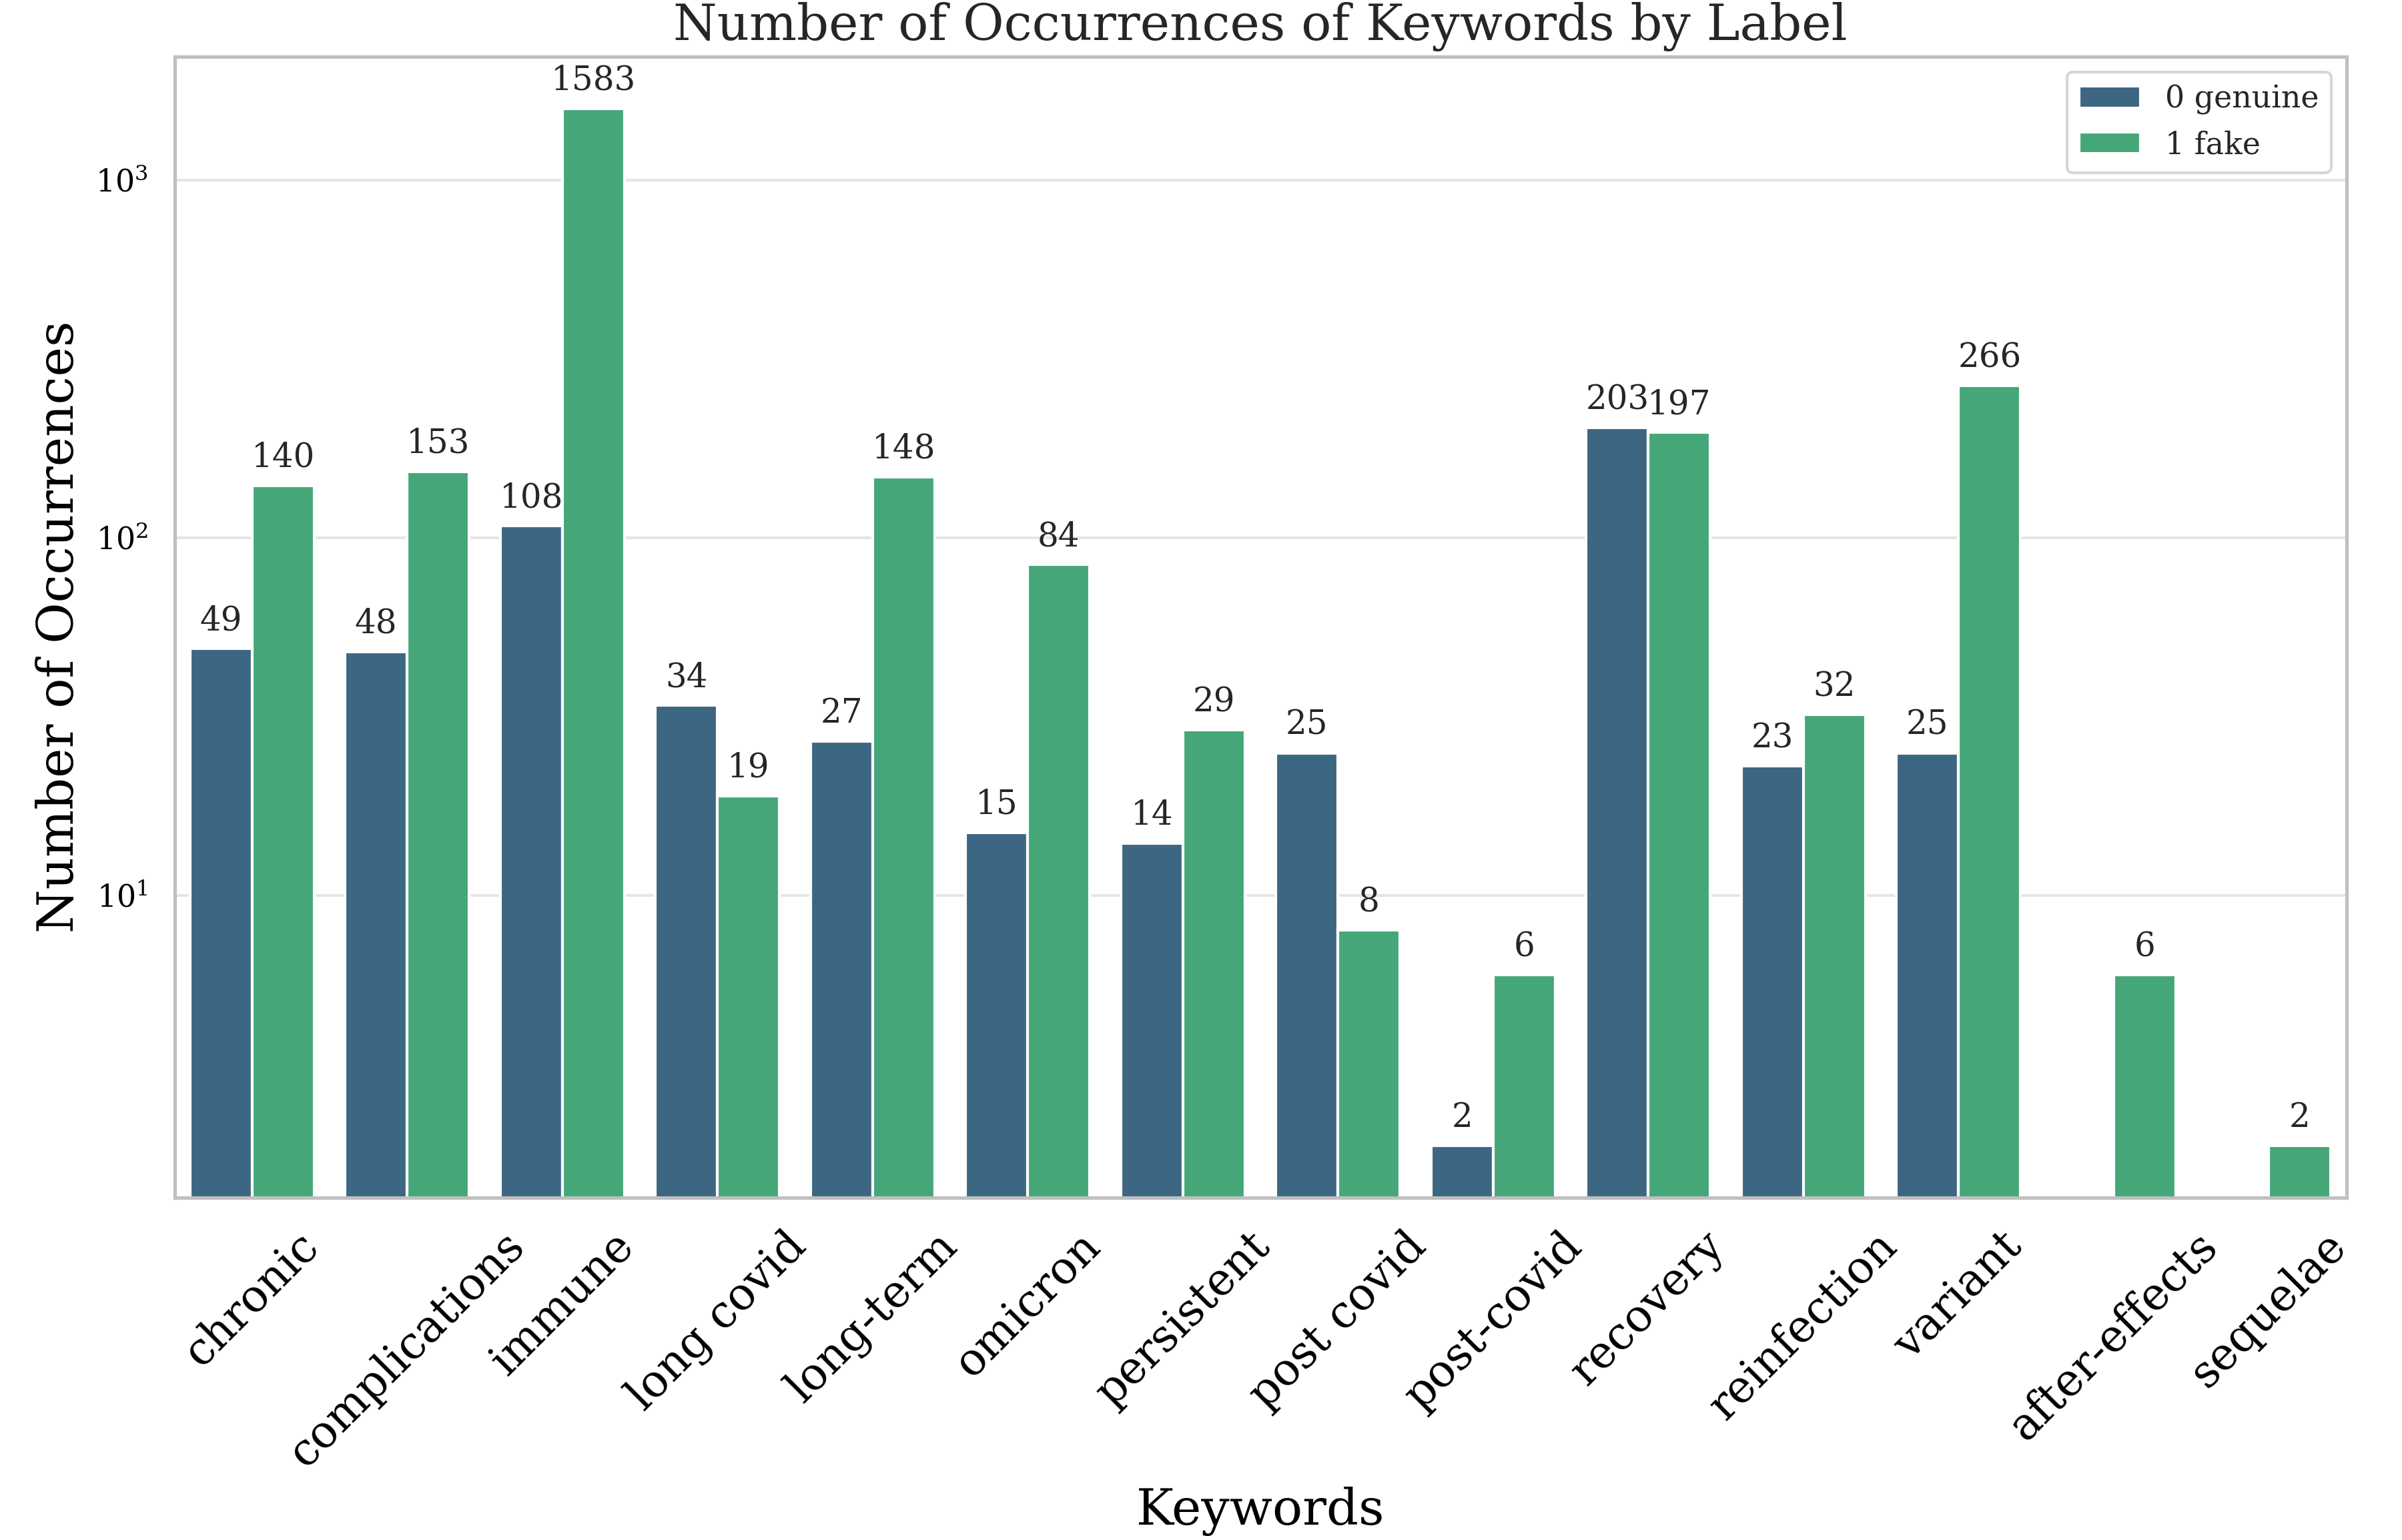
\includegraphics[width=1\linewidth]{img/keywords_by_label.png}
    \caption{Number of keywords occurrences by label}
    \label{fig:keywords_by_label}
\end{figure}

\subsection{Sentiment analysis}
To get a deeper insight into the textual data gathered from fact-checking websites and open-source databases, we utilized the package called TextBlob \cite{b16} for sentiment analysis. Sentiment analysis can reveal whether the textual content of an article is negative, positive, or neutral. Moreover, it can estimate the subjectivity of the text, indicating whether the claim is based on facts or the writer's opinions. \\

\textbf{Polarity:}
Using the TextBlob package, we obtained polarity values ranging from -1 to 1, representing the sentiment from entirely negative to totally positive.To differentiate various sentiment degrees, we categorized sentiments based on polarity into five groups as follows:
\begin{itemize}
\item Strongly Negative: -1 $\leq$ Polarity $<$ -0.5
\item Slightly Negative: -0.5 $\leq$ Polarity $<$ -0.1
\item Neutral: -0.1 $\leq$ Polarity $<$ 0.1
\item Slightly Positive: 0.1 $\leq$ Polarity $<$ 0.5
\item Strongly Positive: 0.5 $\leq$ Polarity $\leq$ 1
\end{itemize}

As Fig. \ref {fig:sentiment} shows, most content is primarily categorized as 'neutral' no matter whether the text is fake or genuine. 65\% of the content in fake texts falls into this category, while 53\% of the content in genuine texts does so. Besides, genuine texts show a higher proportion (36\%) in the "slightly positive" category compared to fake texts (24\%), suggesting that genuine content frequently uses more positive language and favorable terms. The distribution between the two labels is similar in terms of the other sentiment categories ('strongly negative,' 'slightly negative,' and 'strongly positive').\\

\begin{figure}
    \centering
    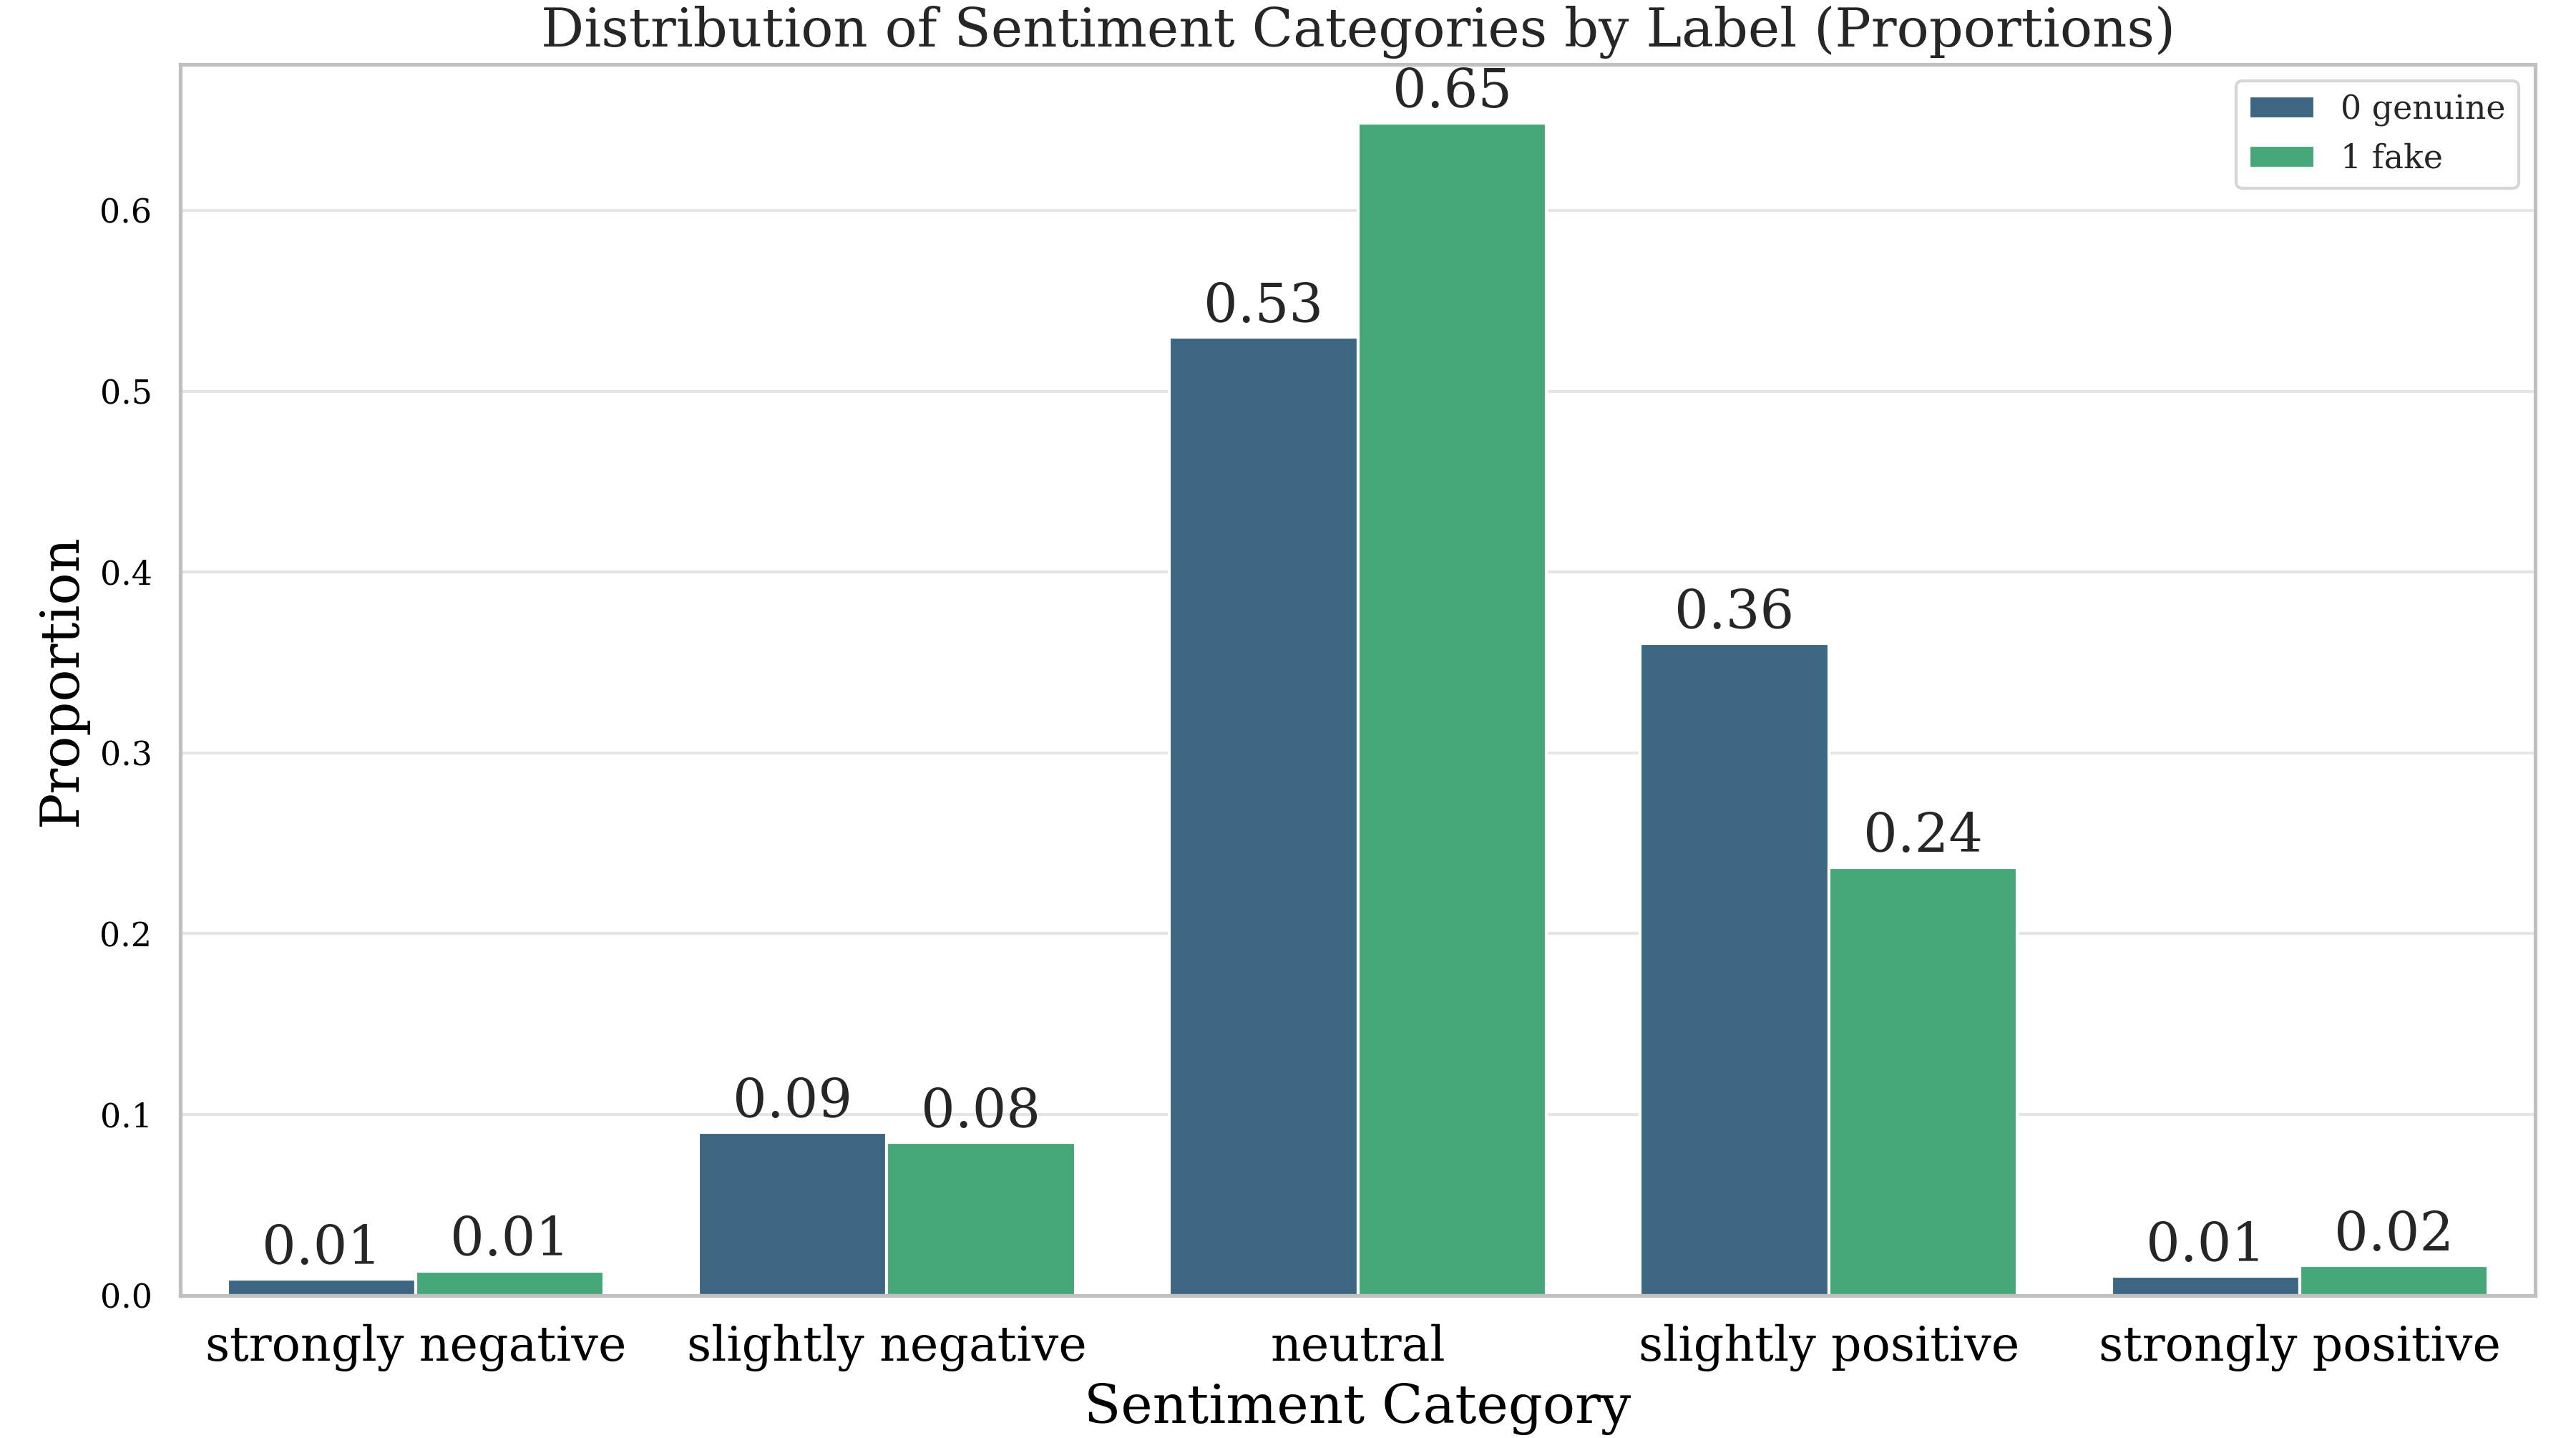
\includegraphics[width=1\linewidth]{img/Sentiment.png}
    \caption{Data distribution (percentage) of different sentiment polarity groups}
    \label{fig:sentiment}
\end{figure}

\textbf{Subjectivity:}
In addition to sentiment analysis, TextBlob provides a subjectivity score ranging from 0 to 1, indicating the degree of subjectivity within the text, ranging from entirely objective to entirely subjective. We categorized the degree of subjectivity into the following five groups:

\begin{itemize}
\item Low Subjectivity: 0 $\leq$ Subjectivity $<$ 0.2
\item Medium-Low Subjectivity: 0.2 $\leq$ Subjectivity $<$ 0.4
\item Medium Subjectivity: 0.4 $\leq$ Subjectivity $<$ 0.6
\item Medium-High Subjectivity: 0.6 $\leq$ Subjectivity $<$ 0.8
\item High Subjectivity: 0.8 $\leq$ Subjectivity $\leq$ 1
\end{itemize}

As illustrated in Fig. \ref {fig:subjectivity}, there is a similarity in the distribution of subjectivity between genuine and fake texts, both primarily falling under the 'medium subjectivity' category. Genuine texts account for 38\% of their content in this category, while fake texts account for 37\%. In the "low subjectivity" category, there is a 5\% higher of fake texts than genuine texts. In the 'medium-high subjectivity' category, genuine texts exceed fake texts by 3\%. \\

These findings emphasize the need for more precise methods to distinguish between genuine and fake news texts because even though some minor differences are observed in the distribution of sentiment polarity and subjectivity between genuine and fake texts, these differences may not serve as definitive classification criteria. Moreover, sentiment analysis faces challenges in natural language understanding, such as accurately identifying sarcasm. Therefore, more precise approaches, such as machine learning algorithms and deep learning models, are required to distinguish genuine from fake news concerning long COVID and reinfections.

\begin{figure}
    \centering
    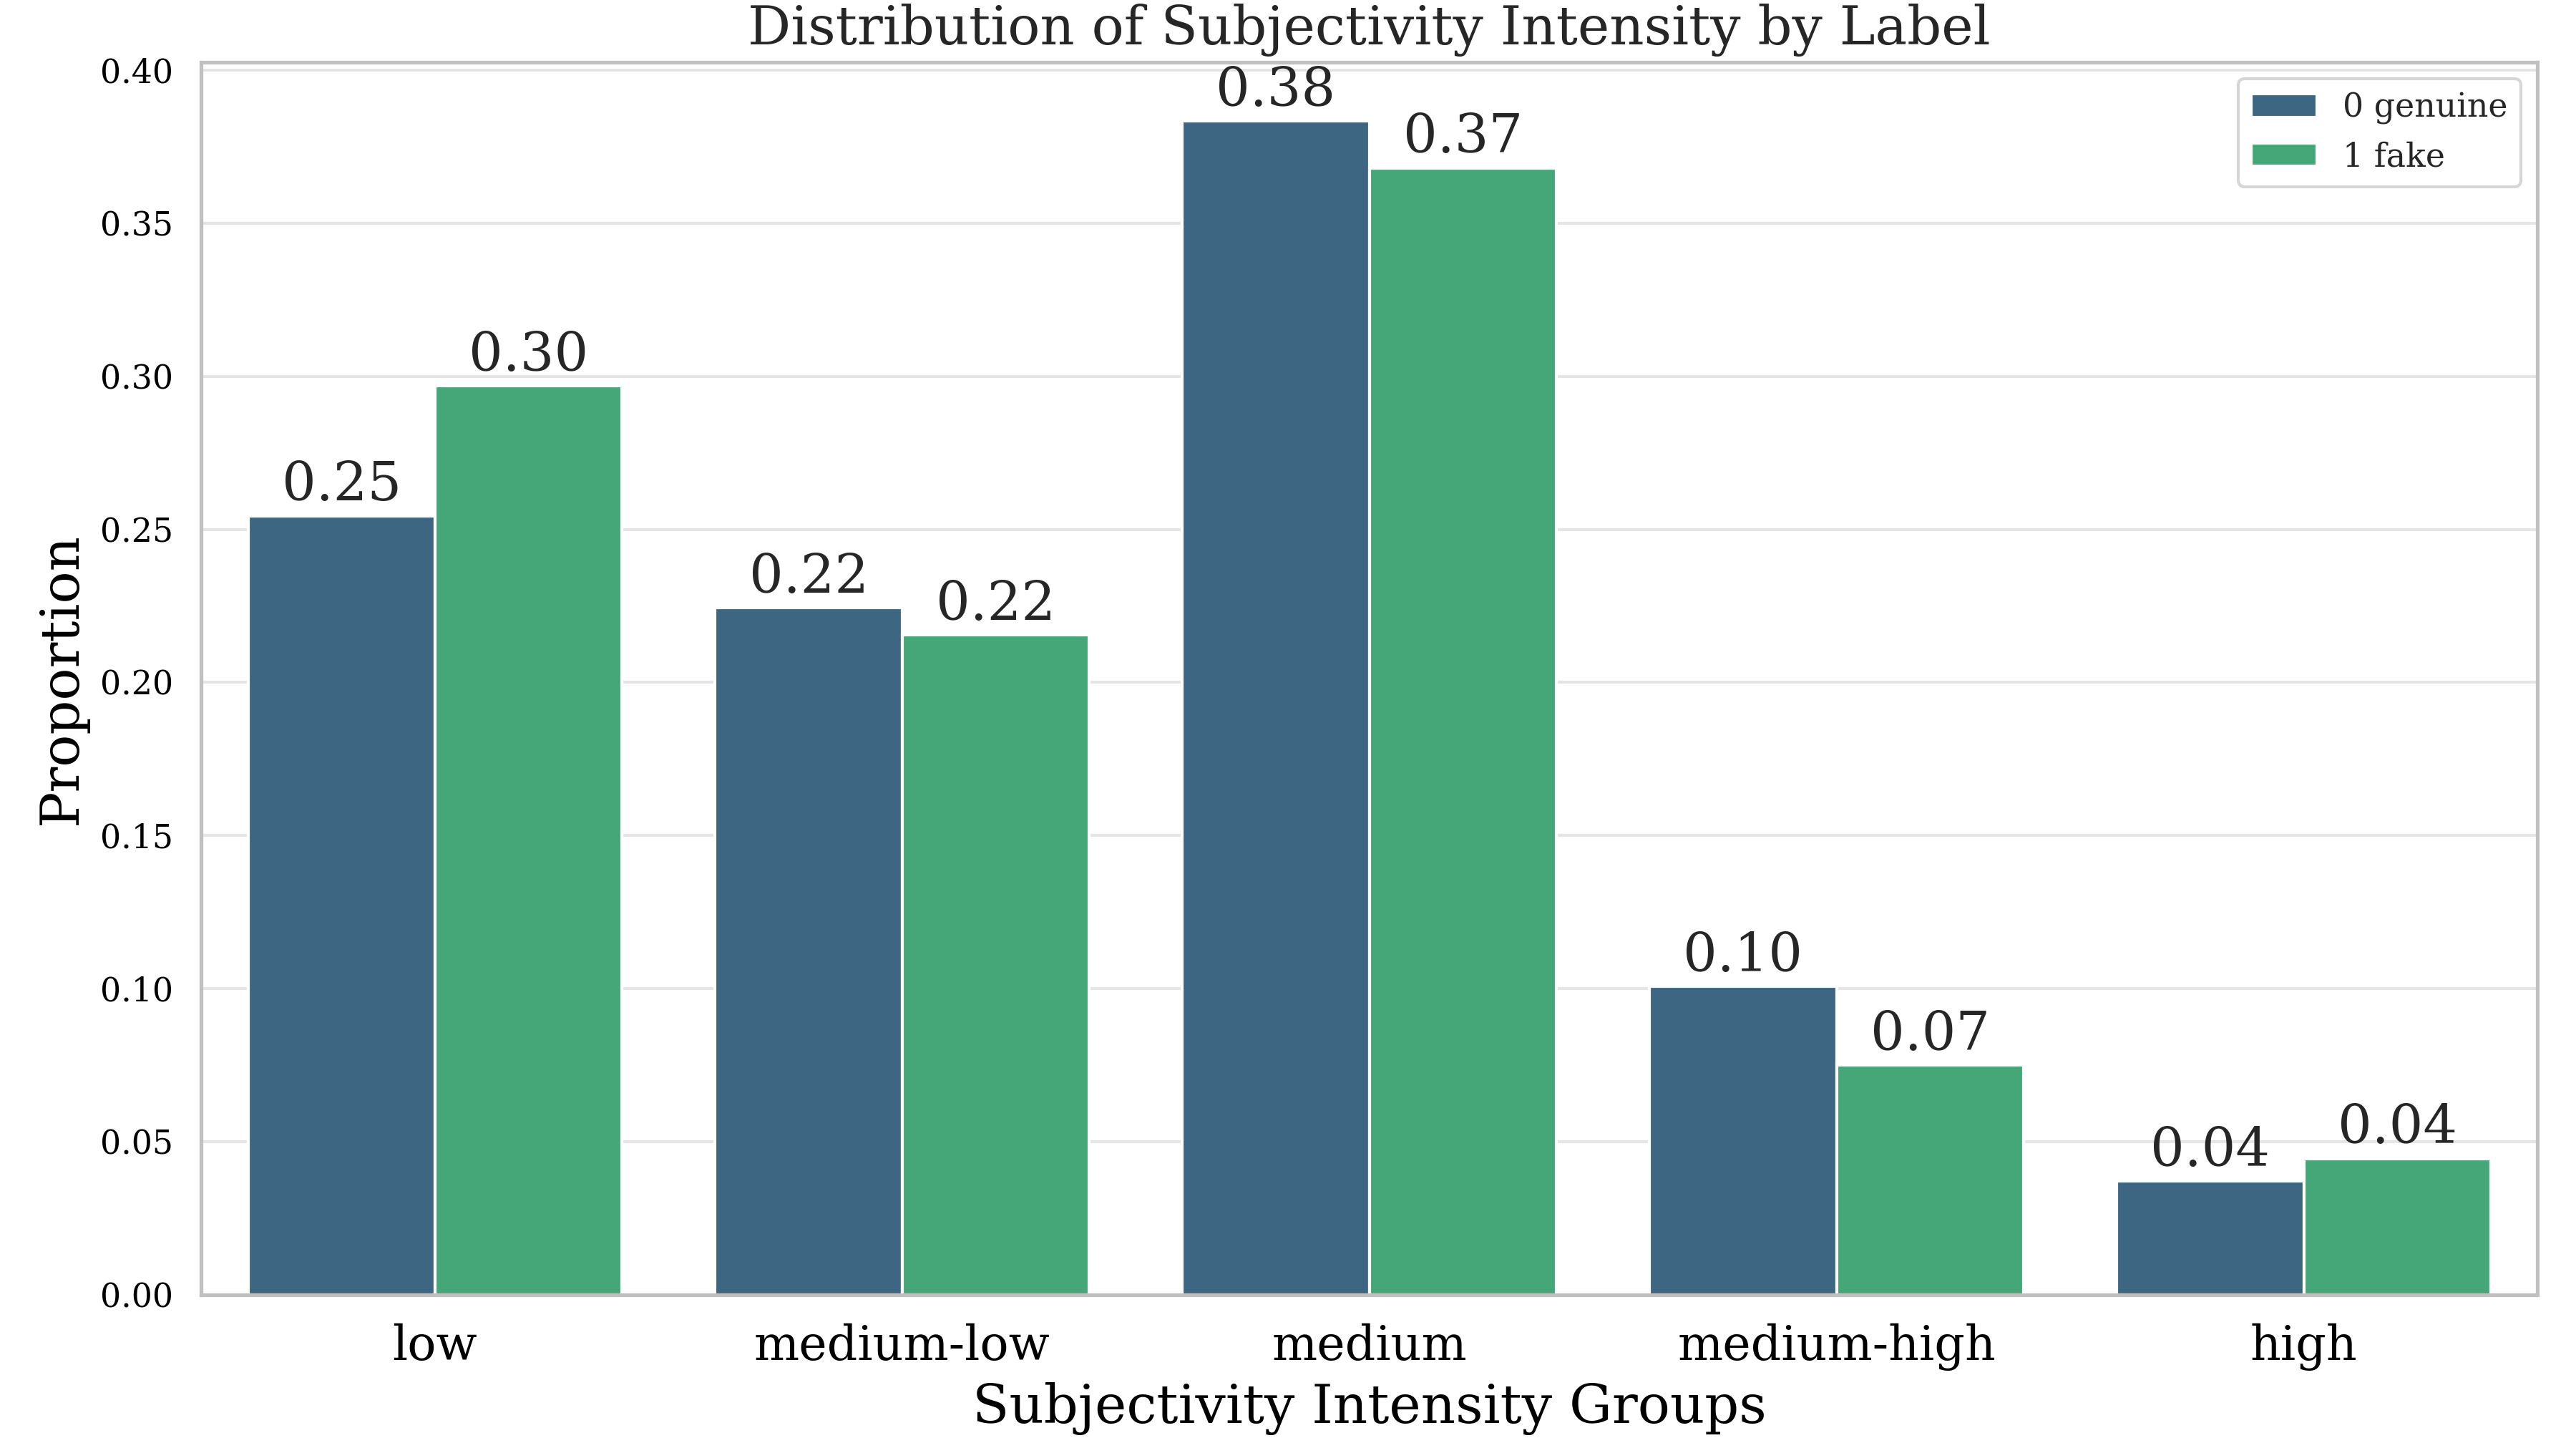
\includegraphics[width=1\linewidth]{img/Subjectivity.png}
    \caption{Data distribution (percentage) of different subjectivity groups}
    \label{fig:subjectivity}
\end{figure}

\section{Models}
In this study, a comprehensive comparison was conducted using various models. Conventional machine learning algorithms that utilized text content or content-based features were employed to establish a baseline. Additionally, attention-based models, from hierarchical neural networks to pre-trained language models, were also explored to take advantage of their advanced capabilities in handling complex textual data. Furthermore, embedding models based on large language models (LLMs) were used to compare the performance between open-source deep models and fee-required models. This approach allowed us to evaluate the effectiveness of different methodologies in distinguishing between genuine and fake news articles, particularly in the context of long COVID and reinfections.

\subsection{TF-IDF with SVM}
To establish a baseline model for text classification, this study initially chose the Support Vector Machine (SVM)\cite{b17}, commonly recognized as a robust baseline model in the field. 
Linear classifiers, such as SVM, provide a straightforward strategy for binary classification tasks by finding the optimal hyperplane that separates two classes in the feature space. 
This study applied the SVM model using uni-gram TF-IDF features generated from the training set data. These features were derived from a bag-of-words approach where each word or token in the text was treated as a separate feature. The TF-IDF (Term Frequency-Inverse Document Frequency) technique was employed to weigh the importance of each word in the document against its frequency in the entire corpus. The TF-IDF score can be represented as the following equation:
\begin{equation}
    TF\text{-}IDF(t,d)=TF(t,d)×IDF(t)
\end{equation}
which consists of two following components:
\begin{equation}
    TF(t,d) = \frac{\text{frequency of the term }\displaystyle t \text{ in the document } \displaystyle d }{\text{number of terms in } \displaystyle d} 
\end{equation}

\begin{equation}
    IDF(t) = log_{e}\left(  \frac{\text{numbers of documents}}{\text{numbers of documents with }t}\right)
\end{equation}
The performance of the SVM classifier was evaluated by comparing its accuracy, precision, recall, and F1-score with those of deep learning models. This comparison helps validate whether deep models are correctly fine-tuned and employed for text classification tasks\cite{b18}.
%https://arxiv.org/pdf/1806.06407
\subsection{Content-based features with XGBoost}
The method combined XGBoost with content-based features, such as frequency of sectarian words, the strength of quoted sources/attribution, and linguistic features, was included in this study\cite{b19}. Generally, articles exhibiting excessively sectarian discourse are deemed less credible. The frequency of sectarian words was calculated by dividing the number of sectarian words by the total number of words in each article.
The strength of source attribution is crucial for determining the trustworthiness of information. This feature measures how well sources are quoted or attributed in the news. Strong and clear source attributions in news articles might enhance credibility.
Additionally, the frequency of assertive verbs, which indicate the degree of certainty in a statement, and factive verbs, which presuppose the truth of a proposition, were measured. High frequencies of these verbs can provide insights into the tone and reliability.
However, due to the limitations of our collected data, the inconsistency score, which measures the consistency of information within and across articles, could not be computed. Therefore, our comparison focused solely on content-based features. These extracted features were then used to train an XGBoost model.

\subsection{HAN}
Hierarchical Attention Networks (HAN)\cite{b20} incorporate attention mechanisms at multiple levels, specifically at the word and sentence levels, to capture diverse hierarchical structures of documents. The authors employed Recurrent Neural Networks (RNNs) combined with word-attention and sentence-attention layers for text classification. This architecture shown in Fig. \ref{fig:HAN} yielded state-of-the-art results across six datasets.

\begin{figure}
    \centering
    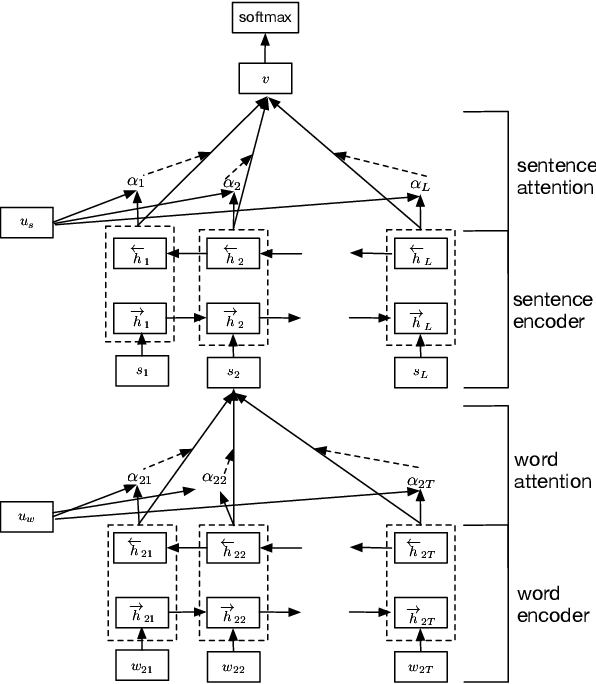
\includegraphics[width=1\linewidth]{img/HAN.png}
    \caption{The architecture of Hierarchical Attention Networks (HAN)\cite{b20}}
    \label{fig:HAN}
\end{figure}

\subsection{BERT}
Bidirectional Encoder Representations from Transformers (BERT)\cite{b21} was a state-of-the-art pre-trained language model based on the Transformer\cite{b22} architecture developed by Google in 2018. It has been trained on massive volumes of text data using masked language modeling and next-sentence prediction techniques. Through self-attention mechanisms, BERT can generate contextualized word representations by considering each word's surrounding context. This contextual information helps BERT to understand the meaning of words in a given sentence more accurately. Due to its robustness and effectiveness, BERT has become one of the most popular and widely used language models in NLP fields. It finds applications across various NLP tasks such as classification, named entity recognition, and question answering.

\subsection{RoBERTa}
In 2019, Facebook introduced the Robustly Optimized BERT Pretraining Approach (RoBERTa)\cite{b23} as an enhancement to the BERT model. RoBERTa was trained on a significantly larger dataset than BERT, allowing it to capture a more comprehensive understanding of language. Unlike BERT, RoBERTa eliminated the next sentence prediction task during pretraining, focusing solely on masked language modeling. Additionally, RoBERTa implemented optimization techniques such as dynamic masking and training with larger batch sizes to improve its performance further. In comparative studies by Facebook, RoBERTa outperformed BERT across various NLP tasks.

\subsection{DeBERTa}
Decoding-enhanced BERT with Disentangled Attention (DeBERTa)\cite{b24}  introduced a novel attention mechanism known as "disentangled attention" to improve upon the original self-attention mechanism. Additionally, it employs the mask decoder and incorporates token absolute positioning to enhance sequence information capturing and pre-training. These enhancements strengthen the model's understanding of text structure and context. In evaluations across various NLP tasks, DeBERTa has demonstrated superior performance to other pre-trained models like BERT and RoBERTa, demonstrating its effectiveness and advancements in NLP research.

\subsection{XLNet}
Introduced by Google in 2019, XLNet\cite{b25} is a pre-trained language model that introduced the concept of "permutation language modeling." This approach aimed to enhance bidirectional contextual understanding within language models. With the Transformer-XL architecture trained on extensive text data, XLNet conquered challenges related to understanding long texts. Furthermore, XLNet overcame certain limitations observed during pre-training from BERT, exhibiting its superior performance compared to other pre-trained language models like RoBERTa and BERT across multiple NLP benchmark tasks.

\subsection{LLMs}
The recent success of large language models (LLMs) has significantly impacted applications within the field of NLP. This study used OpenAI's "text-embedding-ada-002"\cite{b26} and Google's Gemini embedding models\cite{b27} to transform the training set data into embedding. Embedding captures various attributes of a word through vectors, which are lists of floating-point numbers. The relationship between two vectors is measured by their distance, where small distances indicate high relevance and large distances indicate low relevance. Words with similar meanings are typically close to each other in the embedding space. Additionally, arithmetic operations can be performed on word embeddings to yield meaningful results. For instance, the embedding of 'king' - the embedding of 'man' + the embedding of 'woman' is approximately equal to the embedding of 'queen'. Fig. \ref{fig:ada_embedding} shows the visualized embedding of text-embedding-ada-002 using t-SNE\cite{b28}\\

\begin{figure}
    \centering
    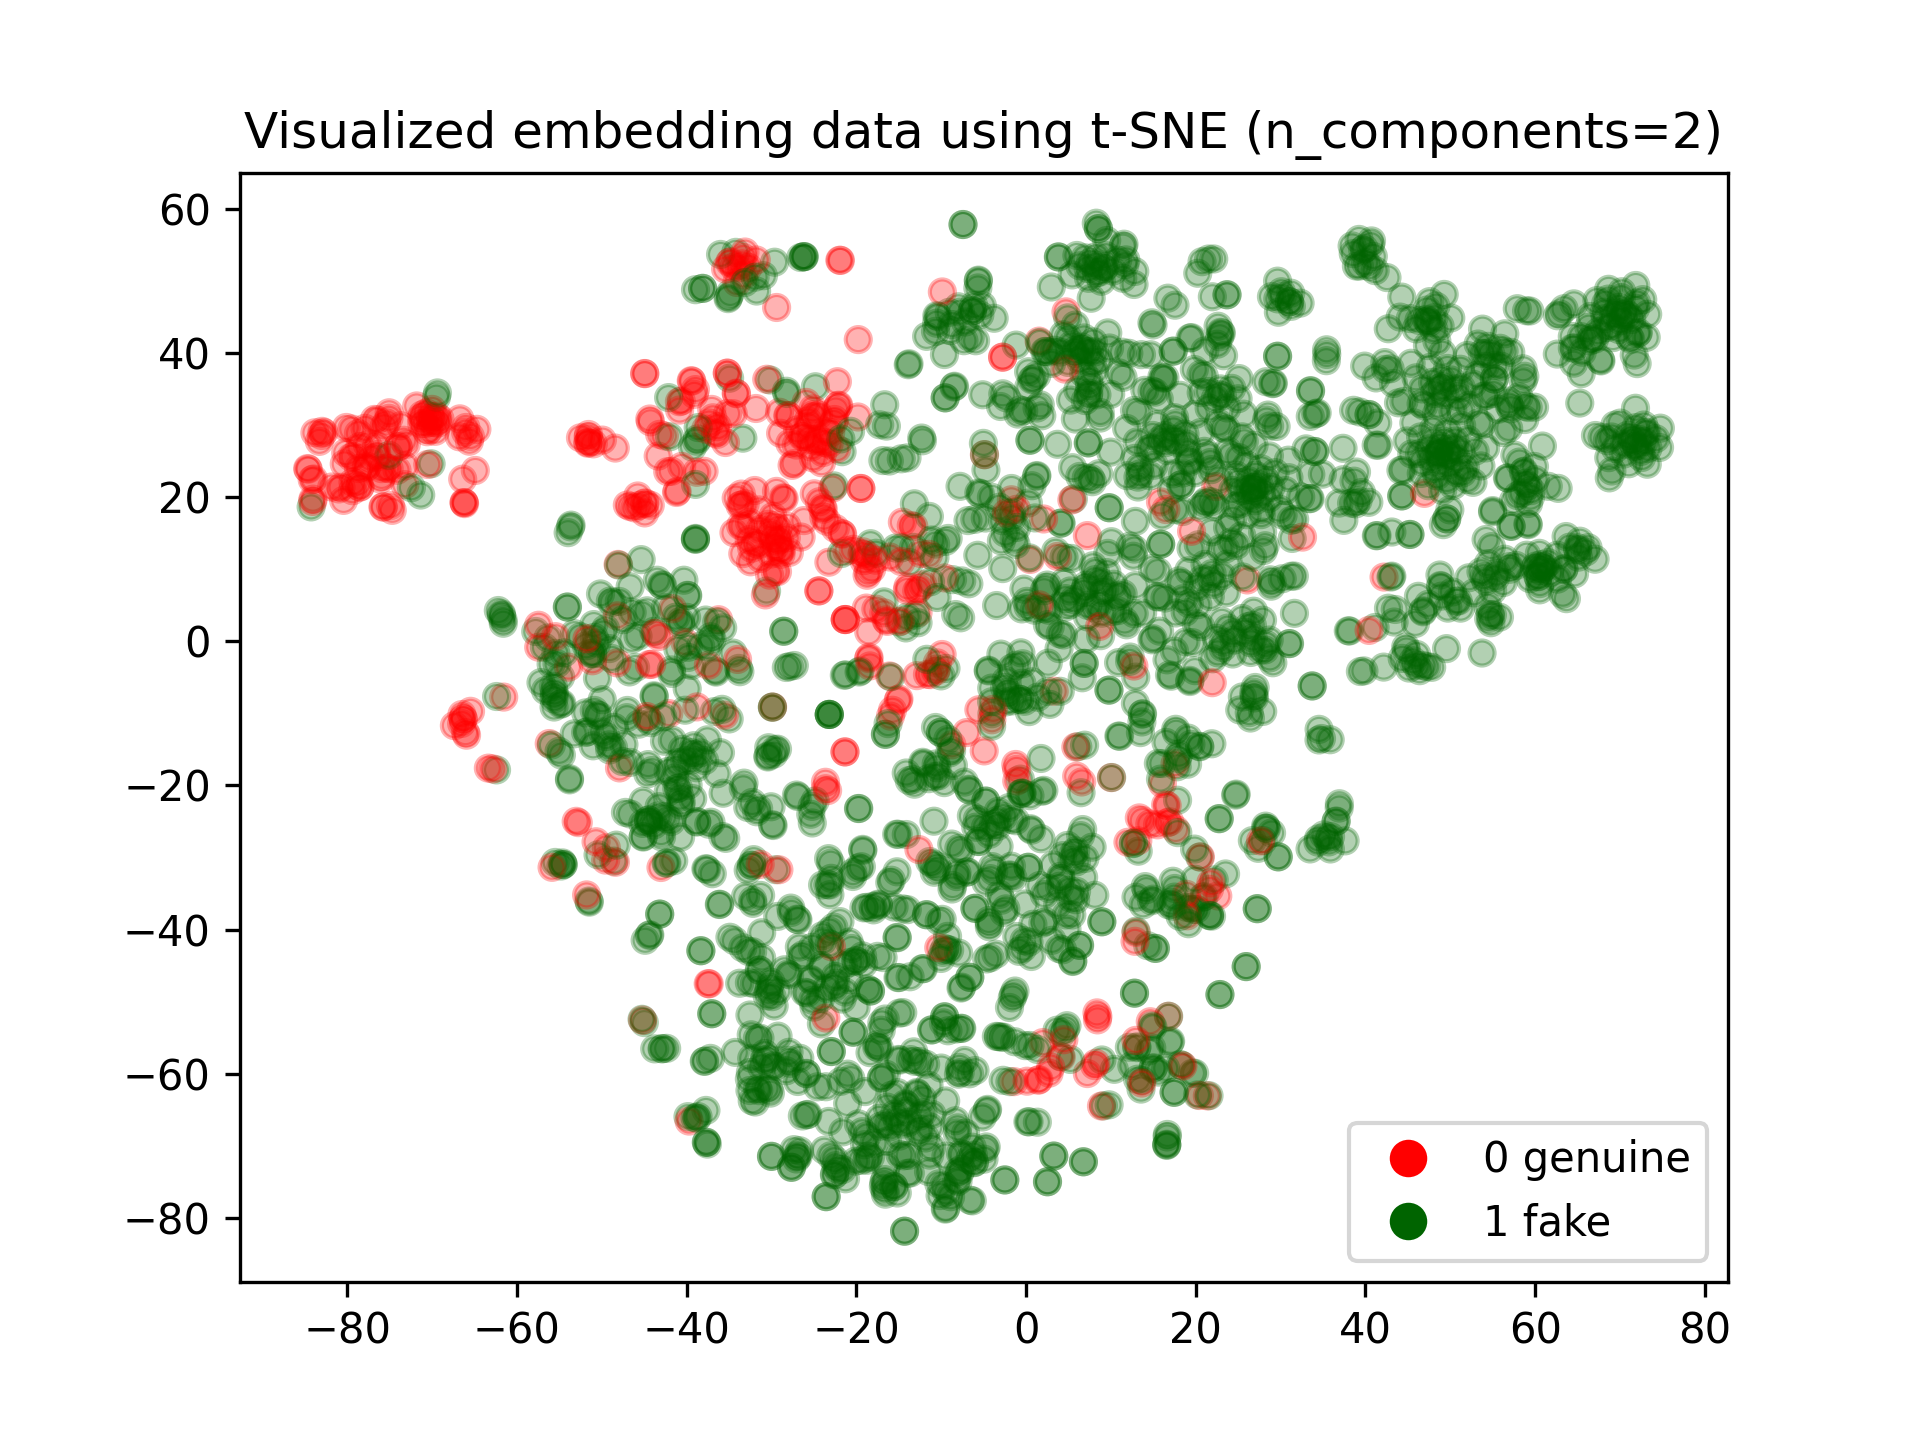
\includegraphics[width=1\linewidth]{img/ada_embedding.png}
    \caption{Visualization of text-embedding-ada-002 model using t-SNE}
    \label{fig:ada_embedding}
\end{figure}

These embeddings were then used as features with the machine learning method, such as SVM, for training. Incorporating knowledge from large language models with the training dataset enhances the accuracy of text classification predictions.
Additionally, OpenAI's GPT-4\cite{b29}, considered the state-of-the-art LLM, was directly employed to infer the texts in the test set. This procedure enables us to compare the performance of LLMs with the other methods in the study.

\section{Ensemble Methods}
Ensemble learning, a technique that combines the strengths of individual models, aims to generate predictions that surpass those of any single model. Traditional ensemble methods include soft voting and hard voting. Soft voting involves averaging the probabilities predicted by multiple classifiers and selecting the class with the highest average probability as the final prediction. On the other hand, hard voting selects the class with the majority of votes according to the hard labels from individual classifiers.\\

\subsection{Fuzzy rank-based ensemble method}
This study employed an approach to enhance prediction performance by combining the Gompertz function into ensemble learning techniques. Specifically, a fuzzy rank-based ensemble technique\cite{b30} was employed, which first considered each classifier's confidence in its predictions for each test case. This differs from conventional ensemble methods, such as average or weighted average rules, which assign pre-defined weights to classifiers. The re-parameterized Gompertz function(Fig. \ref{fig:Gompertz}) was included to compute the fuzzy ranks of each pre-trained model for detection. This method considers each model's predictions' uncertainty and confidence levels, leading to more precise results. To further enhance performance, PLMs like RoBERTa, DeBERTa, and XLNet were combined. These PLMs bring advanced language understanding capabilities to the ensemble, further improving the results.\\
\begin{figure}
    \centering
    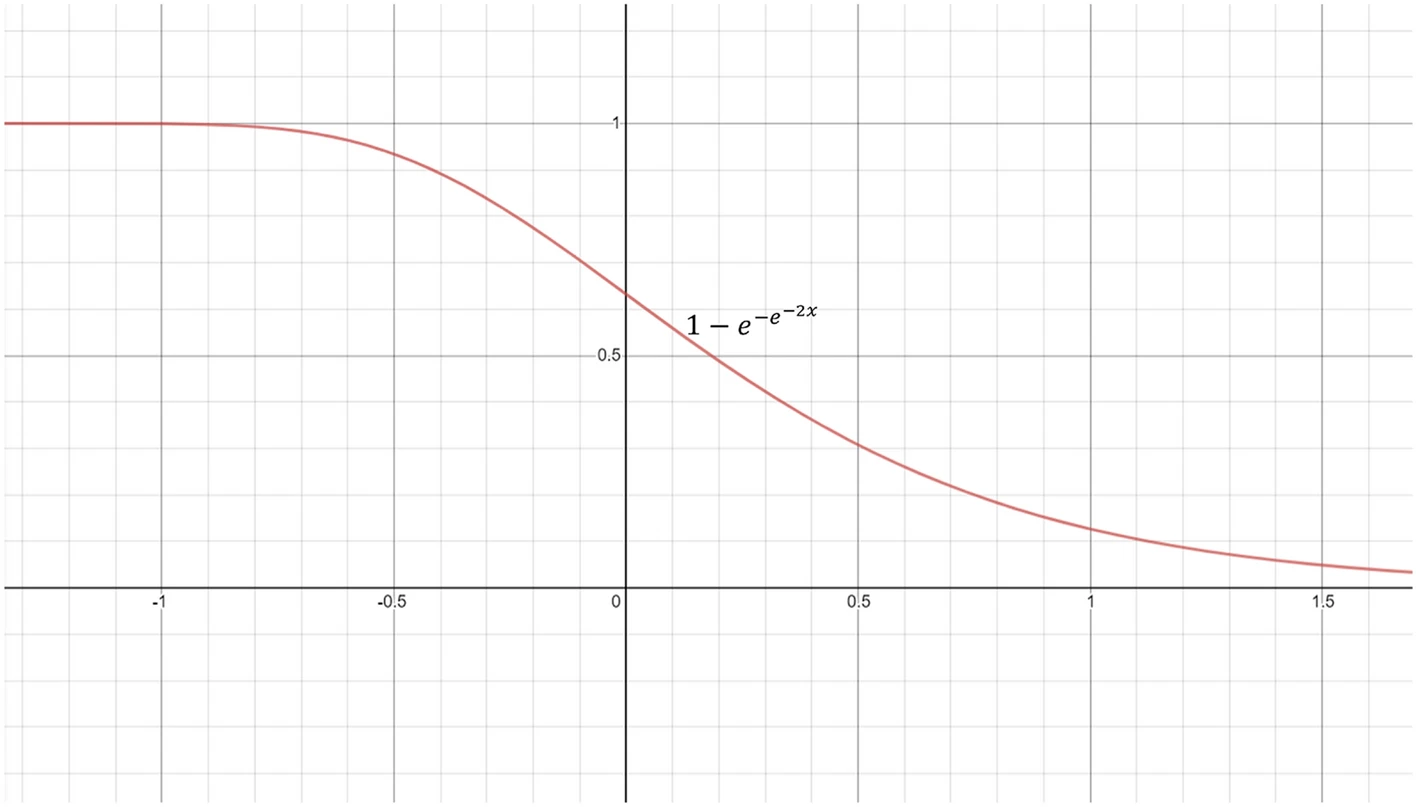
\includegraphics[width=1\linewidth]{img/Gompertz.png}
    \caption{The re-parameterized Gompertz function used in the fuzzy rank-based fusion method.\cite{b30}}
    \label{fig:Gompertz}
\end{figure}

Finally, the predictions of the three models (RoBERTa, DeBERTa, and XLNet) were fused using the fuzzy method, as illustrated in Fig. \ref{fig:process of proposed method}, providing the detailed process of the proposed method.

\begin{figure}
    \centering
    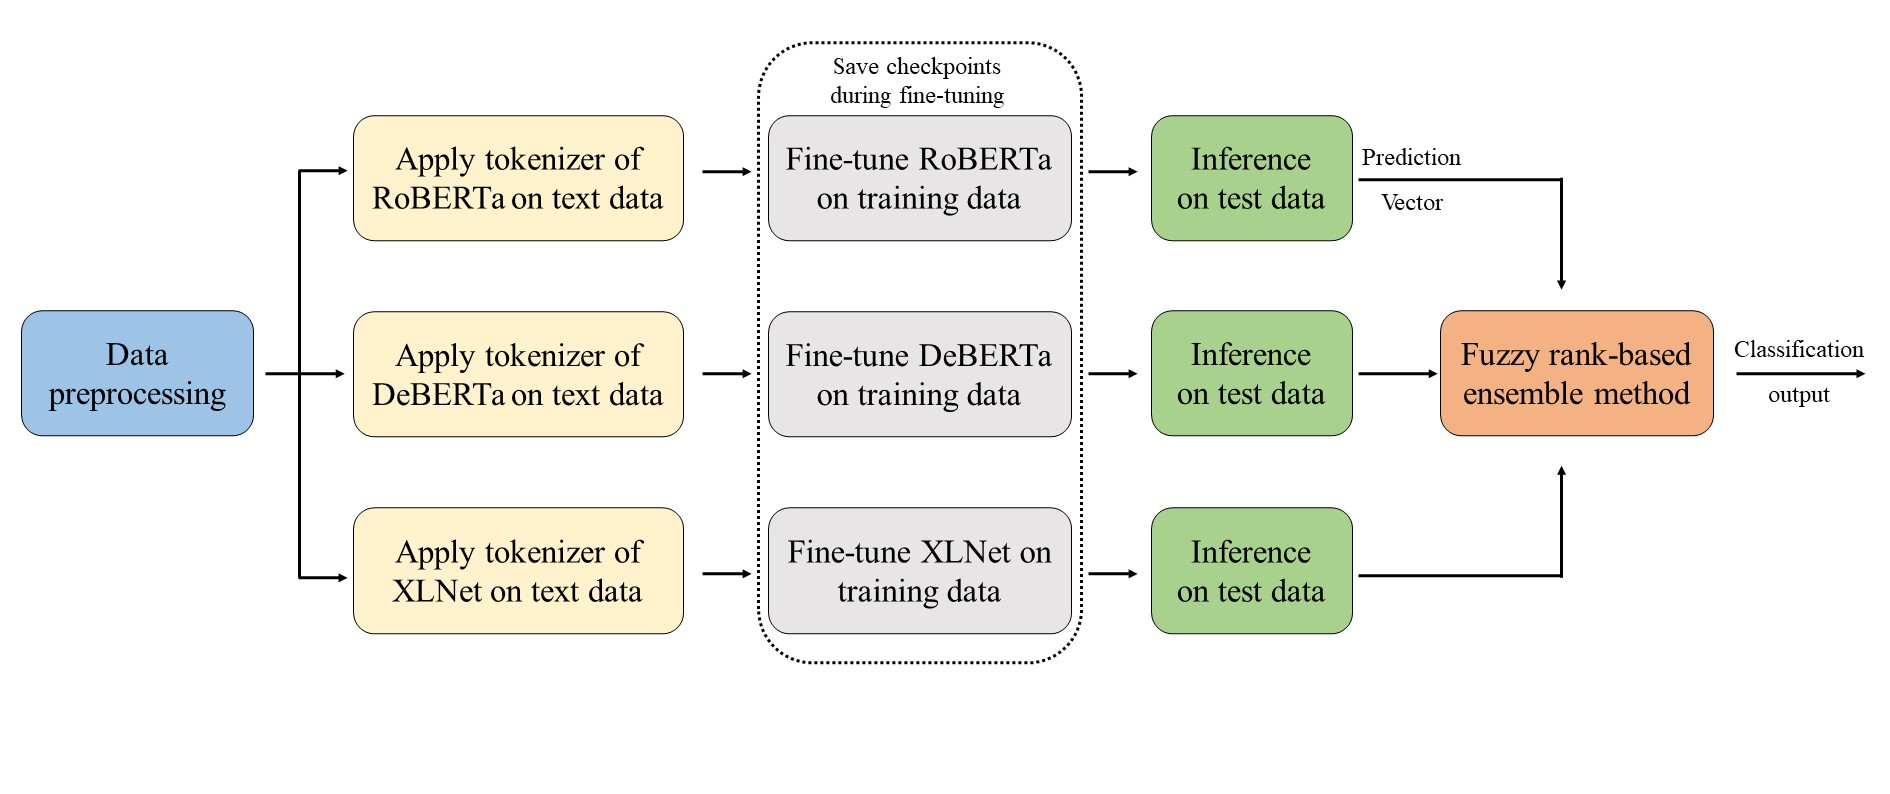
\includegraphics[width=1\linewidth]{img/process of proposed method.JPG}
    \caption{Flowchart of the fuzzy ensemble process using multiple language models.}
    \label{fig:process of proposed method}
\end{figure}

\subsection{Soft voting with content-based features}
The soft voting predicted probabilities were obtained from the RoBERTa, DeBERTa, and XLNet models. Each model assigned a probability to each class for a given instance, which was then averaged. Three content-based features described in Section 3.5.2 were incorporated into the soft voting ensemble method to compare the performance with the fuzzy method. These features were used to train an XGBoost model for final prediction (Fig. \ref{fig:process of content-based features method}). This strategy, which merged soft voting output with content-based features, was aimed at enhancing performance by providing additional context and detailed information, thereby improving classification accuracy. 

\begin{figure}
    \centering
    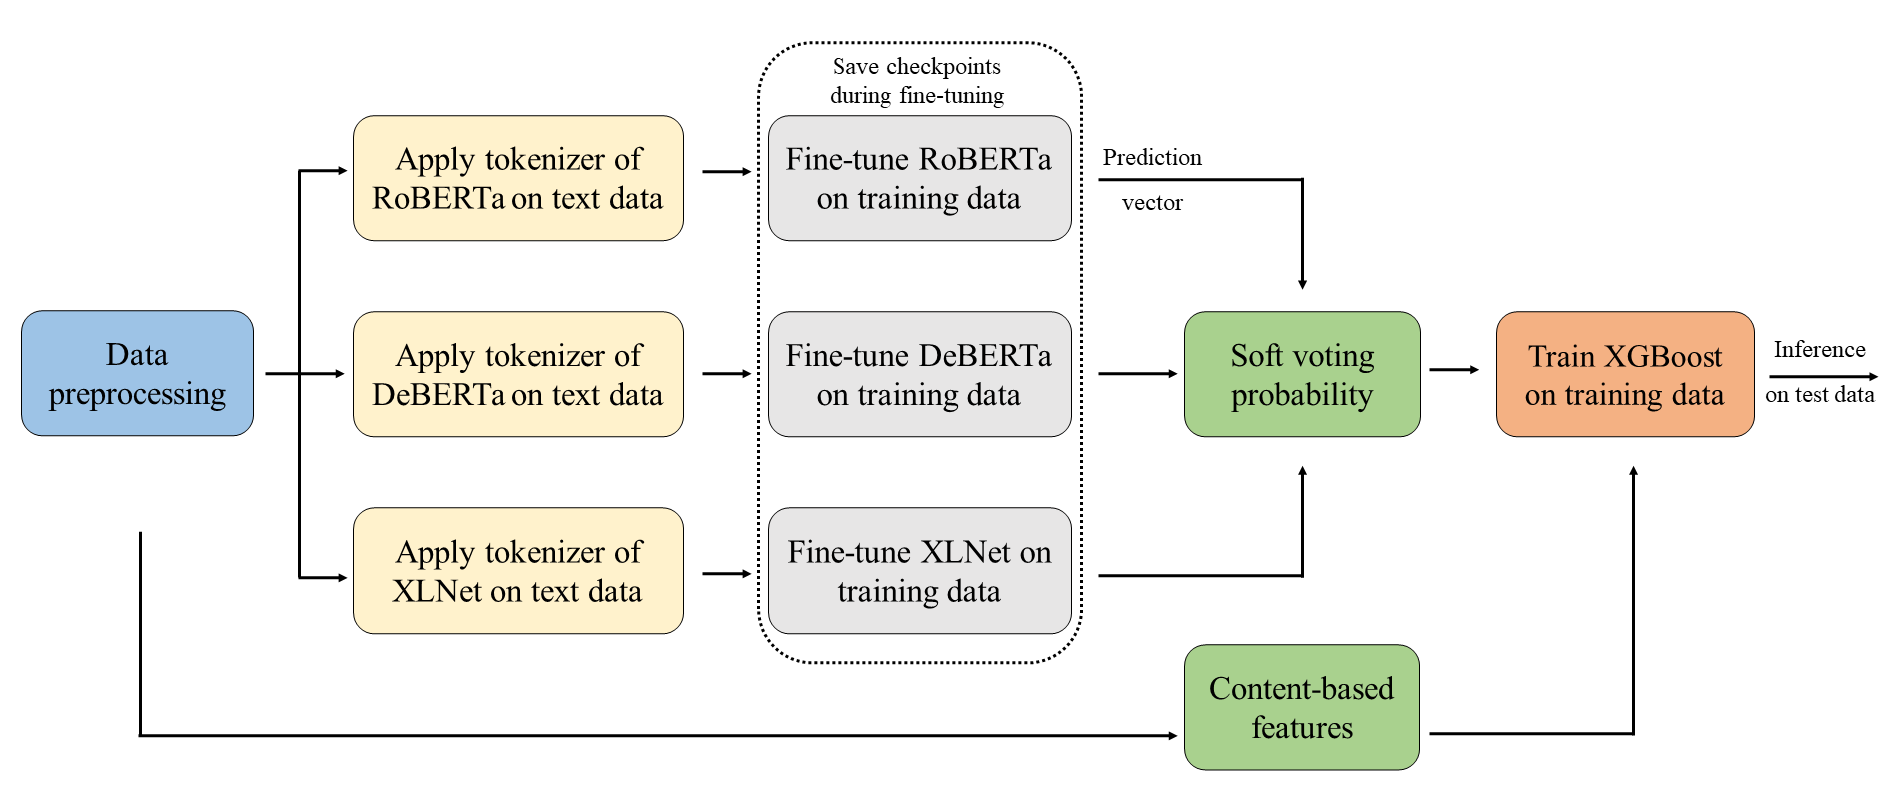
\includegraphics[width=1\linewidth]{img/soft voting with content-based features.png}
    \caption{Flowchart of training XGBoost with soft voting vector and content-based features.}
    \label{fig:process of content-based features method}
\end{figure}
